\chapter{Projet : emploi du templates}

Le but initial du projet ``Emploi du temps'' était de recréer un emploi du temps visuel pour n'importe quel étudiant (ou personnel) de l'UTC, à la manière de celui disponible sur l'ENT\footnote{\url{https://webapplis.utc.fr/edt/index.html}}. Cet emploi du temps se devait d'être un minimum responsive (affichable correctement sur mobile, de manière agréable pour l'utilisateur, sans qu'il ait besoin de zoomer ou dézoomer par exemple). Par ailleurs, ce projet reposait sur l'utilisation d'une API fournie par l'UTC pour récupérer les emplois du temps au format JSON (voir explications plus bas).

\medskip

\noindent De plus, d'autres objectifs supplémentaires nous ont été donnés:
\begin{itemize}
  \item Pouvoir afficher simultanément plusieurs emplois du temps
  \item Vérifier la disponibilité de l'API de l'UTC
\end{itemize}
En plus de ces objectifs secondaires, nous avons rajouté quelques fonctionnalités, détaillées plus bas.

\section{Choix technologiques}

Nous avons décidé de faire notre \textit{back-end} en PHP, avec un \textit{front-end} en HTML, CSS et JavaScript. Au départ nous voulions utiliser des bibliothèques ou \textit{frameworks} (pour le \textit{back-end} ou le \textit{front-end}), dans le but de nous faciliter certaines tâches puis finalement nous avons décidé de tout faire ``à la main'', autant pour le challenge que pour avoir plus de contrôle. De plus, cela nous a permis d'approfondir nos connaissances dans ces langages. Bien trop de personnes savent utiliser un \textit{framework} et non le langage associé. Pour toutes ces raisons, nous avons voulu coder notre projet sans bibliothèque.

\medskip

Concernant les versions, notre projet repose sur une version de PHP >= 5.6 (il a tout du moins été développé et testé sur PHP 5.6, mais il est probable qu'il fonctionne tout de même sur une version inférieure). Quant aux navigateurs web, le projet requiert des fonctions très récentes de JavaScript. Le projet a été testé sur Firefox 45.0 et Google Chrome 49. Il est également probable que le projet fonctionne sur des versions antérieures.

\section{Architecture du projet}

Le code HTML est servi par un script PHP. Ce code HTML appelle ensuite une feuille de style CSS pour embellir l'affichage. Le code HTML contient du code JavaScript intégré (car de petite taille, nous n'avons pas voulu le mettre dans un autre fichier bien que cela soit plus ``propre'').

\section{Fonctionnement}

\begin{figure}[h]
    \centering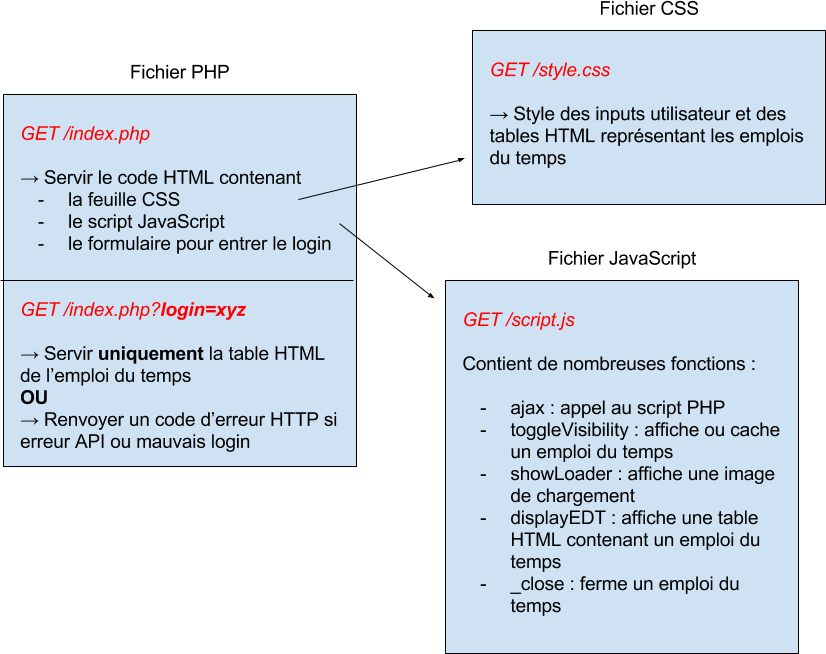
\includegraphics[width=1.00\textwidth]{images/arch.png}
    \caption{Architecture du projet}
\end{figure}

Le JavaScript fera un appel à notre fichier PHP pour récupérer l'emploi du temps d'un étudiant, en transmettant dans la requête son \textit{login}. La réponse contient à nouveau directement du code HTML qui sera ``inclu'' dans notre page actuellement affichée grâce à JavaScript. Il y a quelques éléments visuels de \textit{feedback} (mauvais \textit{login}, API indisponible, etc).

\medskip

Le code PHP, à la reception d'une requête HTTP contenant un paramètre \lstinline{GET}, va aller faire une requête sur l'API de l'UTC\footnote{\url{https://webapplis.utc.fr/Edt_ent_rest/myedt/result?login=<login>}} afin de récupérer l'emploi du temps correspondant au \textit{login}. Cet emploi du temps, servi sous le format JSON, va être traité par notre code PHP afin d'obtenir en résultat final une \lstinline{<table>} HTML. Le code PHP va envoyer ce code HTML final en réponse à la requête envoyé par le JavaScript.

\medskip

Le JavaScript va inclure directement dans la page la table HTML reçue en réponse. Ainsi, il nous est très facile d'afficher plusieurs emplois du temps les uns à la suite des autres. Chaque requête avec un \textit{login} nous permet de récuperer un table HTML qu'il nous suffit de rajouter à la suite, dans notre page couramment affichée.

\section{Résultat final}

\begin{figure}[H]
    \centering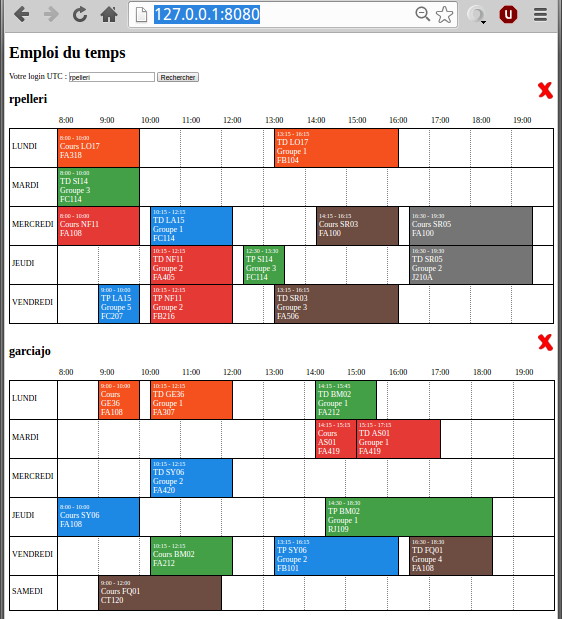
\includegraphics[width=1.00\textwidth]{images/edt.png}
    \caption{Emploi du temps}
\end{figure}


\section{Difficultés rencontrées}
